%2multibyte Version: 5.50.0.2953 CodePage: 1252
% green
% blue
% orange
% purple
% red
% resets numbering each section

\ifdefined\extendedversion\else
  \PassOptionsToClass{handout}{beamer}
\fi
\documentclass[xcolor=x11names,compress,aspectratio=169]{beamer}%
\usepackage{amsmath}
\usepackage{amsfonts}
\usepackage{amssymb}
\usepackage{graphicx}
\usepackage{tikz}
\usepackage{pgfplots}
\usepackage{dcolumn}%
\setcounter{MaxMatrixCols}{30}
%TCIDATA{OutputFilter=latex2.dll}
%TCIDATA{Version=5.50.0.2953}
%TCIDATA{Codepage=1252}
%TCIDATA{CSTFile=beamer.cst}
%TCIDATA{Created=Monday, May 13, 2013 15:44:12}
%TCIDATA{LastRevised=Monday, November 24, 2025 11:45:24}
%TCIDATA{<META NAME="GraphicsSave" CONTENT="32">}
%TCIDATA{<META NAME="SaveForMode" CONTENT="1">}
%TCIDATA{BibliographyScheme=Manual}
%TCIDATA{<META NAME="DocumentShell" CONTENT="Other Documents\SW\Slides - Beamer">}
%TCIDATA{Language=American English}
%BeginMSIPreambleData
\providecommand{\U}[1]{\protect\rule{.1in}{.1in}}
%EndMSIPreambleData
\pgfplotsset{compat=1.18}
\usepgfplotslibrary{groupplots}
%\usepackage{etex} %vers l'infini et au-dela
\usepackage{minted}
\beamertemplatenavigationsymbolsempty
\usepackage[utf8]{inputenc} 
\usepackage[T1]{fontenc} % pour taper les lettres accentuees
%\usepackage[francais, english]{babel} %le rapport est en franÁais 
\usepackage{amsthm,amssymb,amsbsy,amsmath,amsfonts,amscd,mathrsfs}
\usepackage{geometry} %pour la modification des marges
%\usepackage{fancyhdr} %pour modification des pieds de page
%\usepackage{lastpage} %numero de la derniËre page
\usepackage{lmodern}
\usepackage{lscape} % Pour pouvoir activer le mode landscape
\usepackage{booktabs} %tableaux
\usepackage{float}	%pour forcer le placement des images.
\usepackage{graphicx} %pour afficher des images
\usepackage{longtable} %tables sur plusieurs pages
\usepackage{animate} %transformer des gifs
\usepackage{caption}
\captionsetup{labelformat=simple}
\setbeamertemplate{caption}[numbered]
\setbeamerfont{caption}{size=\scriptsize}
\usepackage[scriptsize]{subfigure}
\usepackage{multirow} 			%fusionner lignes
\usepackage{tikz}
\usepackage{adjustbox}
\usetikzlibrary{arrows,positioning}
\usetikzlibrary{mindmap,trees,shadows,backgrounds}
\usepackage{tabularx}
\usepackage{verbatim}%insertion de code
\usepackage{listings}
\usepackage{dsfont} % Pour les lettres mathematiques
\usepackage{hyperref} %pour que les references soient des liens hypertextes
\usepackage{natbib}
\usepackage{bibentry}
\usepackage{color}
\definecolor{bg}{rgb}{0.95,0.95,0.95}

\def\LECTURENAME{Mod\'elisation, estimation, simulation des risques climatiques}
\def\DIPLOMA{Master in Economics, 2$^{nd}$ year}
\def\UNIV{Ecole Polytechnique}
\def\WEBPAGE{\href{http://vermandel.fr/btm/}{http://vermandel.fr/btm}}
\def\SHORTNAME{Modélisation, estimation, simulation des risques climatiques}



%\usepackage{mathpazo}
\usepackage{multimedia}
\usepackage{dcolumn}
\usepackage{mathtools}
\usepackage{xspace}
\usepackage{array}%

\usepackage{graphicx}

\definecolor{light-gray}{gray}{0.85}
\usepackage{ragged2e} % Pour justifier
\definecolor{bleu}{RGB}{0,129,188}
\definecolor{rouge}{RGB}{238,50,78}
\definecolor{orange}{RGB}{255,100,0}
\definecolor{vert}{RGB}{0,157,87}
\newtheorem{hypothese}{Hypoth\`ese}
\newtheorem{remarque}{Hypoth\`ese}
\newtheorem{theoreme}{Th\'eor\`eme}[section]
\newtheorem{definitionDeux}{D\'efinition}[section]
\newcommand{\iid}{\stackrel{\mathrm{iid}}{\sim}}
\usepackage[official,right]{eurosym} % symbols euro
\usepackage{gensymb} % symbole degre \degre
\usepackage{eurosym} % symbole euro
\usepackage{rotating}
\usepackage{multicol}

% Bibliographie
%\usepackage{bib entry}
%\nobibliography*
%\let\newblock\relax

%\usepackage[notocbib]{apacite}
%\usepackage[style=apa]{biblatex}
%\usepackage[round]{natbib}
%\usepackage[style=authoryear]{biblatex}
%\usepackage[backend=bibtex, style=authoryear-comp]{biblatex}
%\usepackage{biblatex}
%\renewcommand*{\bibfont}{\scriptsize} % Pour avoir la biblio en plus petit
%\usepackage{apacite}
%\bibliographystyle{apacite}

\justifying %on justifie le texte du document
\definecolor{deepblue}{RGB}{0,129,188}
\definecolor{deepblue2}{RGB}{158, 64, 57}
\definecolor{deepblue3}{RGB}{245, 84, 66}


% Pour l'annexe (http://tex.stackexchange.com/questions/2541/beamer-frame-numbering-in-appendix)
\newcommand{\backupbegin}{
   \newcounter{framenumberappendix}
   \setcounter{framenumberappendix}{\value{framenumber}}
}
\newcommand{\backupend}{
   \addtocounter{framenumberappendix}{-\value{framenumber}}
   \addtocounter{framenumber}{\value{framenumberappendix}} 
}

%\usepackage{epstopdf}
%\epstopdfDeclareGraphicsRule{.gif}{png}{.png}{%
%  convert gif:#1 png:\OutputFile
%}
%\AppendGraphicsExtensions{.gif}

% A NE PAS UTILISER !
%\let\olditem=\item% 
%\renewcommand{\item}{\olditem \justifying}%

\justifying

%\graphicspath{{../images}}


\usepackage{dcolumn}


% THEME %
\usetheme{Frankfurt}
\useoutertheme[subsection=false,shadow]{miniframes}

\addtobeamertemplate{background canvas}{\transfade[duration=.3]}{}

% Fonts
%\usefonttheme[onlymath]{serif}
%\usefonttheme{structuresmallcapsserif}
%\usefonttheme[onlymath]{mathserif}
%\usefonttheme{serif}
\setbeamerfont{section in head/foot}{size=\tiny, shape=\normalfont}
\setbeamerfont{subsection in toc}{shape=\normalfont, size = \scriptsize}
\setbeamerfont{section in toc}{size = \small, shape=\normalfont}
% Colours
\setbeamercolor{section in head/foot}{fg=black, bg=gray!5}
\setbeamercolor{frametitle}{bg=white, fg=black}
\setbeamercolor{lower separation line head}{bg=black!5}

\setbeamertemplate{sections/subsections in toc}[square]
\setbeamertemplate{items}[triangle]
\setbeamertemplate{itemize subitem}[triangle]
\setbeamertemplate{itemize subsubitem}[ball]
\setbeamertemplate{enumerate items}[default]
\setbeamertemplate{frametitle}[default][rounded=false,shadow=true]

\setbeamercovered{transparent}



\usepackage{assets/beamerouterthemeEwen}
\usepackage{assets/beamercolorthemeEwen}
\usepackage{assets/beamerhighlight}


\newcommand*\grasO[1]{\textbf{\textcolor{orange}{#1}}} 
\newcommand*\grasR[1]{\textbf{\textcolor{rouge}{#1}}}
\newcommand*\grasV[1]{\textbf{\textcolor{vert}{#1}}} 
\newcommand*\grasB[1]{\textbf{\textcolor{bleu}{#1}}} 


\definecolor{rcp26}{RGB}{39, 55, 122}
\definecolor{rcp45}{RGB}{112, 159, 200}
\definecolor{rcp60}{RGB}{222, 99, 43}
\definecolor{rcp85}{RGB}{205, 16, 32}
\definecolor{dp}{RGB}{181, 73, 60}

\newcommand*\grasRCPa[1]{\textbf{\textcolor{rcp26}{#1}}}
\newcommand*\grasRCPb[1]{\textbf{\textcolor{rcp45}{#1}}} 
\newcommand*\grasRCPc[1]{\textbf{\textcolor{rcp60}{#1}}} 
\newcommand*\grasRCPd[1]{\textbf{\textcolor{rcp85}{#1}}} 
%\newcommand {\red} {\color{red}}
\newcommand {\white} {\color{white}}
%\newcommand {\black} {\color{black}}
\def\Frac#1#2{ #1 \color{red}\above 0.4pt \normalcolor #2}


\usetikzlibrary{decorations}
\usetikzlibrary{decorations.pathmorphing}
\usetikzlibrary{shapes.geometric}
\usetikzlibrary{calc}
\usetikzlibrary{decorations.fractals}
\useoutertheme[subsection=false,shadow]{miniframes}
\useinnertheme{default}
\usefonttheme{serif}
\setbeamerfont{title like}{shape=\scshape}
\setbeamerfont{frametitle}{shape=\scshape}
\setbeamercolor*{lower separation line head}{bg=DeepSkyBlue4}
\setbeamercolor*{normal text}{fg=black,bg=white}
\setbeamercolor*{alerted text}{fg=dp}
\setbeamercolor*{example text}{fg=black}
\setbeamercolor*{structure}{fg=black}
\setbeamercolor*{palette tertiary}{fg=black,bg=black!10}
\setbeamercolor*{palette quaternary}{fg=black,bg=black!10}
\renewcommand{\(}{\begin{columns}}
\renewcommand{\)}{\end{columns}}
\newcommand{\<}[1]{\begin{column}{#1}}
\renewcommand{\>}{\end{column}}
\setbeamertemplate{navigation symbols}{}
\setbeamertemplate{headline}{}
\setbeamertemplate{footline}
{
\leavevmode
\hbox{\begin{beamercolorbox}[wd=1\paperwidth,ht=2.25ex,dp=1ex,center]{title in head/foot}\usebeamerfont{title in head/foot}\hfill\hspace*{12em}\insertshorttitle\hspace*{3em}
\insertframenumber{} / \inserttotalframenumber\hspace*{1ex}
\end{beamercolorbox}}
\vskip0pt
}
\newcommand {\red} {\color{red}}
\newcommand {\black} {\color{black}}
\newcommand{\green}{\color{green}}
\definecolor{deepblue}{RGB}{0,129,188}
\newcommand{\pink}{\color{magenta}}
\newcommand{\blue}{\color{deepblue}}
\hypersetup{
colorlinks = true,citecolor=deepblue3,linkcolor=deepblue2
}
\setbeamercolor{frametitle}{fg=deepblue2,bg=white}
\makeatletter
\AtBeginSection[]
{
\ifnum \value{framenumber}>2
\begin{frame}<beamer>
\frametitle{Plan}
\tableofcontents[currentsection,subsectionstyle=hide]
\end{frame}
\else
\fi
}
\let\oldtextbf\textbf
\renewcommand{\textbf}[1]{\textcolor{dp}{\oldtextbf{#1}}}
\newcommand*\annotatedFigureBoxGOT[2]{\draw[thick,rounded corners,deepblue2] (#1) rectangle (#2);}
\newcommand*\annotatedFigureBoxARR[2]{\draw[->,thick,rounded corners,deepblue2] (#1) -- (#2);}
\newcommand*\annotatedFigureBoxCustom[8]{\draw[#5,thick,rounded corners] (#1) rectangle (#2);\node at (#4) [fill=#6,thick,shape=circle,draw=#7,inner sep=2pt,font=\sffamily,text=#8] {\textbf{#3}};}
\newcommand*\annotatedFigureBox[4]{\annotatedFigureBoxCustom{#1}{#2}{#3}{#4}{deepblue2}{deepblue2}{black}{black}}
\newcommand*\annotatedFigureText[4]{\node[draw=none, anchor=south west, text=#2, inner sep=0, text width=#3\linewidth,font=\sffamily] at (#1){#4};}
\newenvironment {annotatedFigure}[1]{\centering\begin{tikzpicture}
\node[anchor=south west,inner sep=0] (image) at (0,0) { #1};\begin{scope}[x={(image.south east)},y={(image.north west)}]}{\end{scope}\end{tikzpicture}}

\usetikzlibrary{arrows.meta,positioning,overlay-beamer-styles}
\usetheme[numbering=none,progressbar=frametitle]{metropolis}
\setbeamertemplate{footline}{
\hfill\usebeamerfont{page number in head/foot}\insertpagenumber/\insertpresentationendpage\hspace{1em}
}
\usetikzlibrary{arrows.meta, positioning, shapes.misc, fit}
\newenvironment{stepenumerate}{\begin{enumerate}[<+->]}{\end{enumerate}}
\newenvironment{stepitemize}{\begin{itemize}[<+->]}{\end{itemize} }
\newenvironment{stepenumeratewithalert}{\begin{enumerate}[<+-| alert@+>]}{\end{enumerate}}
\newenvironment{stepitemizewithalert}{\begin{itemize}[<+-| alert@+>]}{\end{itemize} }
\newtheorem{assumption}[theorem]{Assumption}
\setlength{\itemsep}{1em}
\definecolor{ssp1}{RGB}{27,158,119}
\definecolor{ssp2}{RGB}{55,126,184}
\definecolor{ssp3}{RGB}{217,95,2}
\definecolor{ssp4}{RGB}{152,78,163}
\definecolor{ssp5}{RGB}{228,26,28}
\definecolor{forc19}{RGB}{255,230,230}
\definecolor{forc26}{RGB}{255,180,180}
\definecolor{forc45}{RGB}{255,120,120}
\definecolor{forc70}{RGB}{220,50,50}
\definecolor{forc85}{RGB}{150,0,0}
\newif\ifshowslide
\showslidefalse  % activate the slide
% Compact is the default: each item list is static.
% The extended wrapper turns lists into progressive overlays for lecture delivery.
\ifdefined\extendedversion
  \let\compactitemize\itemize
  \let\endcompactitemize\enditemize
  \renewenvironment{itemize}{\begin{compactitemize}[<+-| alert@+>]}{\end{compactitemize}}
  \renewenvironment{stepitemize}{\begin{compactitemize}[<+->]}{\end{compactitemize}}
  \renewenvironment{stepitemizewithalert}{\begin{compactitemize}[<+-| alert@+>]}{\end{compactitemize}}
\else
  % Static handout: all list content is fully visible, with no animation fade.
  \renewenvironment{stepitemize}{\begin{itemize}}{\end{itemize}}
  \renewenvironment{stepitemizewithalert}{\begin{itemize}}{\end{itemize}}
  \renewenvironment{stepenumerate}{\begin{enumerate}}{\end{enumerate}}
  \renewenvironment{stepenumeratewithalert}{\begin{enumerate}}{\end{enumerate}}
  \setbeamercovered{transparent=100}
\fi
\begin{document}
%
%TCIMACRO{\TeXButton{GG}{\title[\SHORTNAME]{
%\textsc{\footnotesize\SHORTNAME\\ Session 1\\[0.35em] \Large Introducing an Economic Block}
%\\
%}
%\author{ Gauthier Vermandel\\
%{\footnotesize Ecole polytechnique}}
%\date{}}}%
%BeginExpansion
\title[\SHORTNAME]{
\textsc{\footnotesize\SHORTNAME\\ Session 1\\[0.35em] \Large Introducing an Economic Block}
\\
}
\author{ Gauthier Vermandel\\
{\footnotesize Ecole polytechnique}}
\date{}%
%EndExpansion
%

%TCIMACRO{\TeXButton{BeginFrame}{\begin{frame}}}%
%BeginExpansion
\begin{frame}%
%EndExpansion
%

%TCIMACRO{\TeXButton{\maketitle}{\maketitle}}%
%BeginExpansion
\maketitle
%EndExpansion
%

%TCIMACRO{\TeXButton{Transition: Box Out}{\transboxout}}%
%BeginExpansion
\transboxout
%EndExpansion%
%TCIMACRO{\TeXButton{EndFrame}{\end{frame}}}%
%BeginExpansion
\end{frame}%
%EndExpansion
%

%TCIMACRO{\TeXButton{IF}{\ifshowslide}}%
%BeginExpansion
\ifshowslide
%EndExpansion
%

%TCIMACRO{\TeXButton{BeginFrame}{\begin{frame}}}%
%BeginExpansion
\begin{frame}%
%EndExpansion
%

%TCIMACRO{\QTR{frametitle}{General Schedule}}%
%BeginExpansion
\frametitle{General Schedule}%
%EndExpansion


\begin{itemize}
\item \textbf{Thursday 23th September:} \textit{1:30pm to 6:00 pm with 30 min
break}

\textsf{Basics of Economics and Climate}%
%TCIMACRO{\TeXButton{vspace}{\vspace{1ex}}}%
%BeginExpansion
\vspace{1ex}%
%EndExpansion


\item \textbf{Thursday 30th September:}\textit{ 1:30pm to 6:00 pm with 30 min
break}

\textsf{Simulation of \textsf{Climate Economics} Models}%
%TCIMACRO{\TeXButton{vspace}{\vspace{1ex}}}%
%BeginExpansion
\vspace{1ex}%
%EndExpansion


\item \textbf{Thursday 7th October:}\textit{ 1:30pm to 6:00 pm with 30 min
break}

\textsf{Optimization of Climate Economics Models}
\end{itemize}

%

\[
\left[  \text{Gauthier Vermandel 12h}\right]  \rightarrow\left[
\text{Stephane Girard 12h}\right]  \rightarrow\left[  \text{Michael Allouche
12h}\right]
\]


\textbf{Exam:} 16th December (2 hours).%

%TCIMACRO{\TeXButton{Transition: Box Out}{\transboxout}}%
%BeginExpansion
\transboxout
%EndExpansion%
%TCIMACRO{\TeXButton{EndFrame}{\end{frame}}}%
%BeginExpansion
\end{frame}%
%EndExpansion
%

%TCIMACRO{\TeXButton{EnfIF}{\fi}}%
%BeginExpansion
\fi
%EndExpansion
%

%TCIMACRO{\TeXButton{BeginFrame}{\begin{frame}}}%
%BeginExpansion
\begin{frame}%
%EndExpansion
%

%TCIMACRO{\QTR{frametitle}{Technical requirements}}%
%BeginExpansion
\frametitle{Technical requirements}%
%EndExpansion


\begin{itemize}
\item \textbf{Python} preferably with conda

\textit{if not yet installed, do it now it takes \ \symbol{126}15min}%
%TCIMACRO{\TeXButton{vspace}{\vspace{1ex}}}%
%BeginExpansion
\vspace{1ex}%
%EndExpansion


\begin{itemize}
\item \url{https://anaconda.org/anaconda/conda}%
%TCIMACRO{\TeXButton{vspace}{\vspace{1ex}}}%
%BeginExpansion
\vspace{1ex}%
%EndExpansion


\item Exercises in python are done under \textbf{Jupyter notebooks}%
%TCIMACRO{\TeXButton{vspace}{\vspace{1ex}}}%
%BeginExpansion
\vspace{1ex}%
%EndExpansion


\item All materials are available on Moodle
\url{https://moodle.ip-paris.fr/course/view.php?id=18199}%
%TCIMACRO{\TeXButton{vspace}{\vspace{1ex}}}%
%BeginExpansion
\vspace{1ex}%
%EndExpansion


\item Main python packages:
\end{itemize}
\end{itemize}

\begin{center}
[\textsf{sys}] [\textsf{os}] [\textsf{math}] [\textsf{numpy}] [\textsf{pandas}%
] [\textsf{matplotlib}] [\textsf{pandas}] [\textsf{spicy}]
\end{center}

%

%TCIMACRO{\TeXButton{Transition: Box Out}{\transboxout}}%
%BeginExpansion
\transboxout
%EndExpansion%
%TCIMACRO{\TeXButton{EndFrame}{\end{frame}}}%
%BeginExpansion
\end{frame}%
%EndExpansion
%

%TCIMACRO{\TeXButton{BeginFrame}{\begin{frame}}}%
%BeginExpansion
\begin{frame}%
%EndExpansion
%

%TCIMACRO{\QTR{frametitle}{Schedule of the day}}%
%BeginExpansion
\frametitle{Schedule of the day}%
%EndExpansion


\textbf{Objectives}

\begin{itemize}
\item Understanding the \textbf{basics} of macroeconomic model with saving/consumption.

\item Simulating macroeconomic models .%
%TCIMACRO{\TeXButton{vspace}{\vspace{1ex}}}%
%BeginExpansion
\vspace{1ex}%
%EndExpansion

\end{itemize}

\textbf{Materials:}

\begin{itemize}
\item \textsf{notebook\_session1.ipynb} \textit{optimal growth and saving decisions.}

\item \textsf{growth\_model.pdf} \textit{mathematical formulation and interpretation.}

\item \textsf{OptimalGrowth.py} \textit{python package solving optimal
growth models.}
\end{itemize}

\textbf{Some proofs:}

\begin{itemize}
\item Olivier Loisel's lectures on growth models
[\href{https://olivierloisel.com/macroeconomics/Chapter\%201.pdf}{Lecture I}]
[\href{https://olivierloisel.com/macroeconomics/Chapter\%202.pdf}{Lecture II}]
\end{itemize}

%

%TCIMACRO{\TeXButton{Transition: Box Out}{\transboxout}}%
%BeginExpansion
\transboxout
%EndExpansion%
%TCIMACRO{\TeXButton{EndFrame}{\end{frame}}}%
%BeginExpansion
\end{frame}%
%EndExpansion


\section{Introduction}

%

%TCIMACRO{\TeXButton{BeginFrame}{\begin{frame}}}%
%BeginExpansion
\begin{frame}%
%EndExpansion
%

%TCIMACRO{\QTR{frametitle}{Intro: what is an integrated assessment model?}}%
%BeginExpansion
\frametitle{Intro: what is an integrated assessment model?}%
%EndExpansion


\begin{itemize}
\item \textbf{Definition:} IAMs are a combination of science from different
fields: economics, climate, and energy systems into a unified quantitative
framework. \vspace{0.3cm}

\item \textbf{Purpose:} Provide a tractable way to evaluate long-run
interactions between the economy and the climate. \vspace{0.3cm}

\item \textbf{Institutional use:}

\begin{itemize}
\item \textbf{IPCC} (Intergovernmental Panel on Climate Change) relies on IAMs
to define emission scenarios (e.g. SSP pathways).

\item \textbf{Central banks, NGFS, OECD, IEA, World Bank} use IAM-based tools
for stress testing, policy design, and energy forecasts.
\end{itemize}

\vspace{0.3cm}

\item IAMs are \textbf{quantitative tools} used for scenario design, policy
evaluation, and to inform international climate negotiations.
\end{itemize}

%

%TCIMACRO{\TeXButton{Transition: Box Out}{\transboxout}}%
%BeginExpansion
\transboxout
%EndExpansion%
%TCIMACRO{\TeXButton{EndFrame}{\end{frame}}}%
%BeginExpansion
\end{frame}%
%EndExpansion
%

%TCIMACRO{\TeXButton{BeginFrame}{\begin{frame}}}%
%BeginExpansion
\begin{frame}%
%EndExpansion
%

%TCIMACRO{\QTR{frametitle}{Intro: IAM schematic: economy-climate feedbacks}}%
%BeginExpansion
\frametitle{Intro: IAM schematic: economy-climate feedbacks}%
%EndExpansion


\centering\begin{tikzpicture}[
>=Latex,
box/.style={rounded corners=2mm, draw=ssp2!65, line width=0.7pt,
align=center, font=\footnotesize, text width=33mm, minimum height=24mm,
inner sep=2mm, fill=ssp2!5},
policy/.style={box, draw=ssp1!75, fill=ssp1!7, text width=43mm,
minimum height=16mm},
thinarrow/.style={-Latex, line width=0.9pt, draw=ssp2!85!black},
redarrow/.style={-Latex, line width=1pt, draw=ssp3},
]
% (1) Real economy
\node[box, visible on=<1->] (econ) at (0,0) {\textbf{Real economy}\\[1mm]
$Y_t=F(K_t,A_t,L_t)$\\
Consumption\\and investment};
% (2) Emissions
\node[box, visible on=<2->] (emis) at (4.6,0) {\textbf{Emissions}\\[1mm]
$E_t=g(\mu_t)\,Y_t$};
\draw[thinarrow, visible on=<2->] (econ) -- node[above]{} (emis);
% (3) Carbon & Climate  + red damage feedback to economy
\node[box, visible on=<3->] (clim) at (9.2,0) {\textbf{Carbon \& climate}\\[1mm]
Carbon cycle $\to$ $M_t$\\
Radiative forcing $\to$ $T_t$};
\draw[thinarrow, visible on=<3->] (emis) -- node[above,font=\scriptsize]{GHGs} (clim);
\draw[redarrow, rounded corners=3mm, visible on=<3->]
(clim.south) -- (9.2,-3.5) --
node[below,font=\small,text=ssp3]{Climate damages: lower output / utility}
(0,-3.5) -- (econ.south);
% (4) Policy (last)
\node[policy, visible on=<4->] (policy) at (4.6,-2.5) {\textbf{Policy \& controls}\\[1mm]
Abatement $\mu_t$, carbon price $\tau_t$};
\draw[thinarrow, draw=ssp1!85!black, visible on=<4->]
(policy.north) -- node[right,font=\footnotesize]{reduces intensity} (emis.south);
\draw[thinarrow, draw=ssp1!85!black, rounded corners=2mm, visible on=<4->]
(policy.west) -- (1,-2.5)
-- ([xshift=10mm]econ.south);
\node[anchor=west,align=left,font=\scriptsize,text=ssp1!85!black,
visible on=<4->] at (1.1,-1.65) {abatement\\cost};
\end{tikzpicture}%

%TCIMACRO{\TeXButton{Transition: Box Out}{\transboxout}}%
%BeginExpansion
\transboxout
%EndExpansion%
%TCIMACRO{\TeXButton{EndFrame}{\end{frame}}}%
%BeginExpansion
\end{frame}%
%EndExpansion
%

%TCIMACRO{\TeXButton{BeginFrame}{\begin{frame}}}%
%BeginExpansion
\begin{frame}%
%EndExpansion
%

%TCIMACRO{\QTR{frametitle}{Intro: Illustration of IAM\ output}}%
%BeginExpansion
\frametitle{Intro: Illustration of IAM\ output}%
%EndExpansion


\centering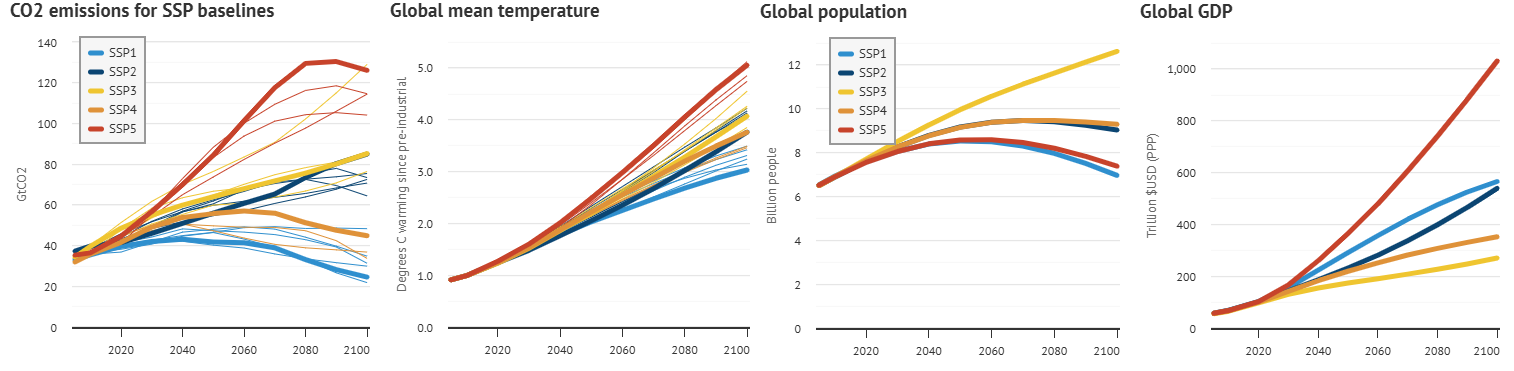
\includegraphics[width=0.95\linewidth]{images/SSPs.png}
\newline\vspace{0.4em} Notes: Illustrative SSP baseline trajectories across
models.
%(edit/add your source here)
%

%TCIMACRO{\TeXButton{Transition: Box Out}{\transboxout}}%
%BeginExpansion
\transboxout
%EndExpansion%
%TCIMACRO{\TeXButton{EndFrame}{\end{frame}}}%
%BeginExpansion
\end{frame}%
%EndExpansion
%

%TCIMACRO{\TeXButton{BeginFrame}{\begin{frame}}}%
%BeginExpansion
\begin{frame}%
%EndExpansion
%

%TCIMACRO{\QTR{frametitle}{Intro: What's inside an IAM?}}%
%BeginExpansion
\frametitle{Intro: What's inside an IAM?}%
%EndExpansion


\begin{itemize}
\item \textbf{Two core blocks} today we treat them as \emph{separate
objects}:\vspace{1ex} \vspace{0.4em}

\begin{itemize}
\item \textbf{Economic block} (2 hours today)\vspace{1ex}\newline\emph{Goal:}
optimal growth / social planner chooses saving (and later abatement).\newline%
\emph{Assumptions (standard in macro, exotic for mathematicians):}
Cobb-Douglas technology, CRRA preferences, competitive pricing, simple capital
law.\vspace{1ex}\newline\emph{Why we use them:} analytical clarity, stability,
(often) uniqueness of equilibrium, and transparent welfare. \vspace{0.6em}

\item \textbf{Climate block} (2 hours today)\vspace{1ex}\newline\emph{Goal:}
map emissions to concentrations, forcing, and temperature.\vspace{1ex}%
\newline\emph{Structure:} few ODEs / linear difference equations (carbon cycle
boxes, 2-box temperature), calibrated to climate science.
\end{itemize}
\end{itemize}

%

%TCIMACRO{\TeXButton{Transition: Box Out}{\transboxout}}%
%BeginExpansion
\transboxout
%EndExpansion%
%TCIMACRO{\TeXButton{EndFrame}{\end{frame}}}%
%BeginExpansion
\end{frame}%
%EndExpansion
%

%TCIMACRO{\TeXButton{BeginFrame}{\begin{frame}}}%
%BeginExpansion
\begin{frame}%
%EndExpansion
%

%TCIMACRO{\QTR{frametitle}{Intro: The big picture: from optimal growth to
%modern IAMs}}%
%BeginExpansion
\frametitle{Intro: The big picture: from optimal growth to modern IAMs}%
%EndExpansion


\begin{itemize}
\item \textbf{Optimal growth tradition} in economics:

\begin{itemize}
\item \textbf{\cite{ramsey1928mathematical}}: how much to save vs. consume
over time?

\item \textbf{\cite{cass1965optimum} - \cite{koopmans1963concept}}: rigorous
optimal growth with capital accumulation, stability and uniqueness of equilibrium.
\end{itemize}

Provides the \emph{benchmark model} of a social planner maximizing
intertemporal welfare.

\vspace{0.4cm}

\item \textbf{\cite{nordhaus1992optimal}}: integrated this framework with
climate science.

\begin{itemize}
\item Extended optimal growth to include \emph{emissions, carbon cycle,
temperature}.

\item Added \emph{damages} and \emph{abatement} as economic choices.

\item Created the \textbf{DICE model}, a prototype IAM (Integrated Assessment Model).
\end{itemize}

\vspace{0.4cm}

\item \textbf{Big picture:} IAMs are the continuation of the optimal growth
tradition, enriched with climate dynamics.
\end{itemize}

%

%TCIMACRO{\TeXButton{Transition: Box Out}{\transboxout}}%
%BeginExpansion
\transboxout
%EndExpansion%
%TCIMACRO{\TeXButton{EndFrame}{\end{frame}}}%
%BeginExpansion
\end{frame}%
%EndExpansion


\section{Core building blocks}%

%TCIMACRO{\TeXButton{BeginFrame}{\begin{frame}}}%
%BeginExpansion
\begin{frame}%
%EndExpansion
%

%TCIMACRO{\QTR{frametitle}{Building Blocks: main ingredients}}%
%BeginExpansion
\frametitle{Building Blocks: main ingredients}%
%EndExpansion


\begin{itemize}
\item \textbf{Discrete time} framework

\begin{itemize}
\item Period length fixed (e.g. annual).

\item Easier to match with economic and climate data.
\end{itemize}

\vspace{0.3cm}

\item \textbf{Notation:} $X_{t}$ denotes the value of variable $X$ in period
$t$. \vspace{0.3cm}

\item \textbf{Centralized economy} (social planner)

\begin{itemize}
\item A single agent (the planner) chooses allocations for society
$\rightarrow$ deterministic optimal control problem.
\end{itemize}

\vspace{0.3cm}

\item \textbf{Aggregate representation}

\begin{itemize}
\item Output, capital, consumption, labor all modeled as aggregate variables.

\item Abstracts from heterogeneity to focus on long-run dynamics.
\end{itemize}
\end{itemize}

%

%TCIMACRO{\TeXButton{Transition: Box Out}{\transboxout}}%
%BeginExpansion
\transboxout
%EndExpansion%
%TCIMACRO{\TeXButton{EndFrame}{\end{frame}}}%
%BeginExpansion
\end{frame}%
%EndExpansion
%

%TCIMACRO{\TeXButton{BeginFrame}{\begin{frame}}}%
%BeginExpansion
\begin{frame}%
%EndExpansion
%

%TCIMACRO{\QTR{frametitle}{Building Blocks: Production function I}}%
%BeginExpansion
\frametitle{Building Blocks: Production function I}%
%EndExpansion


\begin{itemize}
\item \textbf{Gross Domestic Product (GDP)}: total value of goods and services
produced in one period. $\rightarrow$ It is a \textbf{flow}, not a stock.
\vspace{0.3cm}

\item GDP is calculated from a production function $F(\cdot)$ which we define
as \textquotedblleft Cobb-Douglas\textquotedblright:
\[
Y_{t}=F(K_{t},A_{t}L_{t})=A_{t}K_{t}^{\alpha}L_{t}^{1-\alpha}%
\]


\begin{itemize}
\item $Y_{t}\geq0$: output in period $t$ (GDP),

\item $A_{t}\geq0$: productivity (technology),

\item $K_{t}\geq0$: capital,

\item $L_{t}\geq0$: labor,

\item $\alpha\in\lbrack0,1]$: capital share ($\sim0.3$ empirically).
\end{itemize}
\end{itemize}

%

%TCIMACRO{\TeXButton{Transition: Box Out}{\transboxout}}%
%BeginExpansion
\transboxout
%EndExpansion%
%TCIMACRO{\TeXButton{EndFrame}{\end{frame}}}%
%BeginExpansion
\end{frame}%
%EndExpansion
%

%TCIMACRO{\TeXButton{BeginFrame}{\begin{frame}}}%
%BeginExpansion
\begin{frame}%
%EndExpansion
%

%TCIMACRO{\QTR{frametitle}{Building Blocks: Production function II}}%
%BeginExpansion
\frametitle{Building Blocks: Production function II}%
%EndExpansion


Denoting by $k_{t}=\tfrac{K_{t}}{A_{t}L_{t}}$ the stock of capital per
effective-labor unit, we get
\[
\frac{Y_{t}}{A_{t}L_{t}}\;=\;\frac{1}{A_{t}L_{t}}F(K_{t},A_{t}L_{t}%
)\;=\;F(k_{t},1)\;\equiv\;f(k_{t})
\]
\medskip where $f$ has the following properties:

\begin{enumerate}
\item $f:\mathbb{R}^{+}\rightarrow\mathbb{R}^{+},\;k\mapsto f(k)$, with
$f(0)=0$,

\item $f$ is \textbf{strictly increasing}: $\;\forall k\in\mathbb{R}%
^{+},\;f^{\prime}(k)>0$,

\item $f$ is \textbf{strictly concave}: $\;\forall k\in\mathbb{R}%
^{+},\;f^{\prime\prime}(k)<0$,

\item $f$ satisfies the \textbf{Inada conditions}: $\lim_{k\rightarrow
0}f^{\prime}(k)=+\infty$ and $\lim_{k\rightarrow+\infty}f^{\prime}(k)=0$:

\begin{itemize}
\item $\lim_{k\rightarrow0}f^{\prime}(k)$ infinite $f^{\prime}(k)$ guarantees
that it is always worthwhile to accumulate at least some capital: avoid
\textquotedblleft poverty trap\textquotedblright\ at $k=0$

\item $\lim_{k\rightarrow+\infty}f^{\prime}(k)$ prevents infinite growth
simply from capital accumulation alone.
\end{itemize}
\end{enumerate}

%

%TCIMACRO{\TeXButton{Transition: Box Out}{\transboxout}}%
%BeginExpansion
\transboxout
%EndExpansion%
%TCIMACRO{\TeXButton{EndFrame}{\end{frame}}}%
%BeginExpansion
\end{frame}%
%EndExpansion
%

%TCIMACRO{\TeXButton{BeginFrame}{\begin{frame}}}%
%BeginExpansion
\begin{frame}%
%EndExpansion
%

%TCIMACRO{\QTR{frametitle}{Building Blocks: Production function III}}%
%BeginExpansion
\frametitle{Building Blocks: Production function III}%
%EndExpansion


\centering\begin{tikzpicture}
\begin{groupplot}[
group style={group size=2 by 1, horizontal sep=1.7cm},
width=5.8cm, height=4.2cm,
axis lines=left, axis line style={gray!65,-Latex},
title style={font=\small\bfseries},
label style={font=\small},
xtick=\empty, ytick=\empty,
clip=true
]
% ----- Left: f(k) (use f(k)=sqrt(k) as a concave example) -----
\nextgroupplot[
title={Output increases with capital},
xmin=0, xmax=10,
ymin=0, ymax=3.5,
xlabel={$k_t$},
ylabel={$f(k_t)$},
domain=0:10, samples=300
]
\addplot[ssp2, line width=1.5pt] {sqrt(x)};
% origin dots for style similar to your figure
\node[font=\small,text=ssp2] at (axis cs:6,1.4) {$f'(k)>0$};
% optional: light asymptote hint at k=0
% \draw[densely dotted] (axis cs:0,0) -- (axis cs:0,3.3);
% ----- Right: f'(k) = 1/(2 sqrt(k)) -----
\nextgroupplot[
title={Marginal product decreases},
xmin=0, xmax=10,
ymin=0, ymax=2.5,
xlabel={$k_t$},
ylabel={$f'(k_t)$},
domain=0.05:10, samples=300
]
\addplot[ssp3, line width=1.5pt] {1/(2*sqrt(x))};
% show vertical behaviour near zero
\node[font=\small,text=ssp3] at (axis cs:6,1.3) {$f''(k)<0$};
\end{groupplot}
\end{tikzpicture}\par\medskip
{\small Illustration: $f(k)=\sqrt{k}$.\\
More capital raises output, but each additional unit contributes less.}

%TCIMACRO{\TeXButton{Transition: Box Out}{\transboxout}}%
%BeginExpansion
\transboxout
%EndExpansion%
%TCIMACRO{\TeXButton{EndFrame}{\end{frame}}}%
%BeginExpansion
\end{frame}%
%EndExpansion
%

%TCIMACRO{\TeXButton{BeginFrame}{\begin{frame}}}%
%BeginExpansion
\begin{frame}%
%EndExpansion
%

%TCIMACRO{\QTR{frametitle}{Building Blocks: Why Cobb--Douglas?}}%
%BeginExpansion
\frametitle{Building Blocks: Why Cobb--Douglas?}%
%EndExpansion


\begin{itemize}
\item \textbf{Homogeneity of degree 1} (constant returns to scale):
\[
Y(\lambda K,\lambda L)=\lambda Y(K,L)
\]
$\rightarrow$ doubling capital and labor doubles output. \vspace{0.3cm}

\item \textbf{Implications:}

\begin{itemize}
\item Factor shares are constant over time.

\item Each factor has diminishing marginal productivity.

\item Guarantees stability and uniqueness of equilibrium in optimal growth models.
\end{itemize}

\vspace{0.3cm}

\item Widely used in macroeconomics for simplicity and tractability.
\end{itemize}

%

%TCIMACRO{\TeXButton{Transition: Box Out}{\transboxout}}%
%BeginExpansion
\transboxout
%EndExpansion%
%TCIMACRO{\TeXButton{EndFrame}{\end{frame}}}%
%BeginExpansion
\end{frame}%
%EndExpansion
%

%TCIMACRO{\TeXButton{BeginFrame}{\begin{frame}}}%
%BeginExpansion
\begin{frame}%
%EndExpansion
%

%TCIMACRO{\QTR{frametitle}{Building Blocks: GDP\ allocation}}%
%BeginExpansion
\frametitle{Building Blocks: GDP\ allocation}%
%EndExpansion


\begin{itemize}
\item Recall: \textbf{GDP $Y_{t}$} is the total value of goods and services
produced in one period. $\rightarrow$ It is a \textbf{flow}, not a stock.
\vspace{0.3cm}

\item From the \textbf{demand side}, GDP is allocated to:
\[
Y_{t} = C_{t} + I_{t}
\]


\begin{itemize}
\item $C_{t}$: consumption (households, public),

\item $I_{t}$: investment (new machines, buildings, infrastructure).
\end{itemize}

\vspace{0.3cm}

\item Example:

\begin{itemize}
\item A household buying food $\;\to\;$ consumption.

\item A firm building a new factory $\;\to\;$ investment.
\end{itemize}
\end{itemize}

%

%TCIMACRO{\TeXButton{Transition: Box Out}{\transboxout}}%
%BeginExpansion
\transboxout
%EndExpansion%
%TCIMACRO{\TeXButton{EndFrame}{\end{frame}}}%
%BeginExpansion
\end{frame}%
%EndExpansion
%

%TCIMACRO{\TeXButton{BeginFrame}{\begin{frame}}}%
%BeginExpansion
\begin{frame}%
%EndExpansion
%

%TCIMACRO{\QTR{frametitle}{Building Blocks: Capital accumulation}}%
%BeginExpansion
\frametitle{Building Blocks: Capital accumulation}%
%EndExpansion


\begin{itemize}
\item \textbf{Capital dynamics:}
\[
K_{t+1} = (1 - \delta) K_{t} + I_{t}
\]
where:

\begin{itemize}
\item $K_{t}$: stock of capital (machines, factories, infrastructure),

\item $\delta$: depreciation rate (typically $\sim5\%$ per year),

\item $I_{t}$: new investment.
\end{itemize}

\vspace{0.3cm}

\item \textbf{Interpretation:}

\begin{itemize}
\item Each period, a fraction $\delta$ of capital "wears out".

\item Investment replenishes and grows the capital stock.

\item Today's saving $\to$ tomorrow's productive capacity.
\end{itemize}

\vspace{0.3cm}

\item This law of motion is the \textbf{state equation} of the optimal growth model.
\end{itemize}

%

%TCIMACRO{\TeXButton{Transition: Box Out}{\transboxout}}%
%BeginExpansion
\transboxout
%EndExpansion%
%TCIMACRO{\TeXButton{EndFrame}{\end{frame}}}%
%BeginExpansion
\end{frame}%
%EndExpansion
%

%TCIMACRO{\TeXButton{BeginFrame}{\begin{frame}}}%
%BeginExpansion
\begin{frame}%
%EndExpansion
%

%TCIMACRO{\QTR{frametitle}{Building Blocks: Preferences (setup)}}%
%BeginExpansion
\frametitle{Building Blocks: Preferences (setup)}%
%EndExpansion


\begin{itemize}
\item In growth models, we evaluate \textbf{per capita consumption}:
\[
c_{t} = \frac{C_{t}}{L_{t}}
\]
where $C_{t}$ is aggregate consumption, $L_{t}$ is population. \vspace{0.3cm}

\item \textbf{Utility at the individual level}: captures satisfaction from
consumption of goods at date $t$. \vspace{0.3cm}

\item Standard assumption: \textbf{CRRA utility} (constant relative risk
aversion):
\[
U(c_{t}) = \frac{c_{t}^{\,1-\gamma} - 1}{1-\gamma}, \quad\gamma> 0
\]


\begin{itemize}
\item $\gamma$: curvature parameter = risk aversion = $1/$(intertemporal
elasticity of substitution).
\end{itemize}
\end{itemize}

%

%TCIMACRO{\TeXButton{Transition: Box Out}{\transboxout}}%
%BeginExpansion
\transboxout
%EndExpansion%
%TCIMACRO{\TeXButton{EndFrame}{\end{frame}}}%
%BeginExpansion
\end{frame}%
%EndExpansion
%

%TCIMACRO{\TeXButton{BeginFrame}{\begin{frame}}}%
%BeginExpansion
\begin{frame}%
%EndExpansion
%

%TCIMACRO{\QTR{frametitle}{Building Blocks: Preferences II}}%
%BeginExpansion
\frametitle{Building Blocks: Preferences II}%
%EndExpansion


\begin{itemize}
\item $U$: $\mathbb{R}^{+}\rightarrow\mathbb{R}$ (U can take negative values,
what matters is the relative difference)

\item $U$ is strictly increasing: $\forall c\in\mathbb{R}^{+}$, $u^{\prime
}\left(  c\right)  >0$

\item $U$ is strictly concave: $\forall c\in\mathbb{R}^{+}$, $u^{\prime\prime
}\left(  c\right)  <0$

\item $U$ satisfies \textquotedblleft Inada conditions\textquotedblright:
$\lim_{c\rightarrow0}$ $u^{\prime}\left(  c\right)  =+\infty$ and
$\lim_{c\rightarrow+\infty}$ $u^{\prime}\left(  c\right)  =0$

\begin{itemize}
\item Ensures an interior optimum in dynamic optimization problems (no corner solutions).

\item Interpretation: \newline$\lim_{c\rightarrow0}$ $u^{\prime}\left(
c\right)  $ formalizes the idea that\textbf{ starving is infinitely painful}
(so agents avoid it), \newline$\lim_{c\rightarrow+\infty}$ $u^{\prime}\left(
c\right)  $ formalizes satiation: more and \textbf{more consumption eventually
adds negligible utility}.
\end{itemize}
\end{itemize}

%

%TCIMACRO{\TeXButton{Transition: Box Out}{\transboxout}}%
%BeginExpansion
\transboxout
%EndExpansion%
%TCIMACRO{\TeXButton{EndFrame}{\end{frame}}}%
%BeginExpansion
\end{frame}%
%EndExpansion
%

%TCIMACRO{\TeXButton{BeginFrame}{\begin{frame}}}%
%BeginExpansion
\begin{frame}%
%EndExpansion
%

%TCIMACRO{\QTR{frametitle}{Building Blocks: Preferences III}}%
%BeginExpansion
\frametitle{Building Blocks: Preferences III}%
%EndExpansion


\centering\begin{tikzpicture}
\begin{axis}[
width=8cm,height=4.8cm,axis lines=left,
axis line style={gray!65,-Latex},xmin=0,xmax=9,ymin=0,ymax=3.2,
xlabel={Consumption $c$},ylabel={$U(c)$},
xtick=\empty,ytick=\empty,clip=true,
label style={font=\small},domain=0:9,samples=300]
\addplot[ssp2,line width=1.5pt] {sqrt(x)};
\draw[gray!45,densely dashed] (axis cs:1,0) -- (axis cs:1,1);
\draw[gray!45,densely dashed] (axis cs:3,0) -- (axis cs:3,1.73205);
\draw[gray!45,densely dashed] (axis cs:6,0) -- (axis cs:6,2.44949);
\draw[gray!45,densely dashed] (axis cs:8,0) -- (axis cs:8,2.82843);
\addplot[only marks,mark=*,mark size=1.8pt,ssp2]
coordinates {(1,1) (3,1.73205) (6,2.44949) (8,2.82843)};
\draw[ssp3,line width=1pt,<->] (axis cs:1,0.25) --
node[above,font=\scriptsize] {$\Delta c$} (axis cs:3,0.25);
\draw[ssp3,line width=1pt,<->] (axis cs:6,0.25) --
node[above,font=\scriptsize] {$\Delta c$} (axis cs:8,0.25);
\end{axis}
\node[anchor=west,align=left,font=\small,text width=4cm,
text=ssp2!80!black] at (7.2,2)
{$U'(c)>0$\\More is better.\\[5mm]
$U''(c)<0$\\Marginal utility\\decreases.};
\end{tikzpicture}\par\medskip
{\small Equal increases in consumption yield smaller utility gains at higher $c$.\\
Illustration: $U(c)=\sqrt{c}$, up to affine normalization.}

%TCIMACRO{\TeXButton{Transition: Box Out}{\transboxout}}%
%BeginExpansion
\transboxout
%EndExpansion%
%TCIMACRO{\TeXButton{EndFrame}{\end{frame}}}%
%BeginExpansion
\end{frame}%
%EndExpansion
%

%TCIMACRO{\TeXButton{BeginFrame}{\begin{frame}}}%
%BeginExpansion
\begin{frame}%
%EndExpansion
%

%TCIMACRO{\QTR{frametitle}{Building Blocks: Intertemporal welfare}}%
%BeginExpansion
\frametitle{Building Blocks: Intertemporal welfare}%
%EndExpansion


\begin{itemize}
\item The planner values utility flows across time:
\[
W = \sum_{t=0}^{\infty}\beta^{t} \, L_{t} \, U(c_{t})
\]
\vspace{0.3cm}

\item \textbf{Discounting}:
\[
\beta= \frac{1}{1+\rho}, \quad\rho> 0
\]


\begin{itemize}
\item $\rho$: pure rate of time preference.

\item Low $\rho$: future generations valued more (Stern).

\item High $\rho$: more weight on present (Nordhaus).
\end{itemize}

\vspace{0.3cm}

\item Preferences combine two dimensions:

\begin{enumerate}
\item \emph{Across goods}: concavity ($\gamma$) governs curvature of $U(c)$.

\item \emph{Across time}: discounting ($\beta, \rho$) governs how much future
is valued.
\end{enumerate}
\end{itemize}

%

%TCIMACRO{\TeXButton{Transition: Box Out}{\transboxout}}%
%BeginExpansion
\transboxout
%EndExpansion%
%TCIMACRO{\TeXButton{EndFrame}{\end{frame}}}%
%BeginExpansion
\end{frame}%
%EndExpansion
%

%TCIMACRO{\TeXButton{BeginFrame}{\begin{frame}}}%
%BeginExpansion
\begin{frame}%
%EndExpansion
%

%TCIMACRO{\QTR{frametitle}{Building Blocks: Introducing the saving rate}}%
%BeginExpansion
\frametitle{Building Blocks: Introducing the saving rate}%
%EndExpansion


\begin{itemize}
\item Recall the resource identity with $c_{t}=C_{t}/L_{t}$:
\[
Y_{t}=c_{t}L_{t}+I_{t}%
\]
\vspace{0.3cm}

\item Define the \textbf{saving rate} $s_{t}$:
\[
I_{t} = s_{t} Y_{t}, \quad C_{t} = (1-s_{t}) Y_{t}
\]
\vspace{0.3cm}

\item Interpretation:

\begin{itemize}
\item $s_{t}$ is the \textbf{balance-sheet view of GDP}: it tells us how much
of income is devoted to \emph{future capacity} (investment) vs \emph{current
use} (consumption).

\item This simple choice variable links today's output to tomorrow's capital.
\end{itemize}
\end{itemize}

%

%TCIMACRO{\TeXButton{Transition: Box Out}{\transboxout}}%
%BeginExpansion
\transboxout
%EndExpansion%
%TCIMACRO{\TeXButton{EndFrame}{\end{frame}}}%
%BeginExpansion
\end{frame}%
%EndExpansion
%

%TCIMACRO{\TeXButton{BeginFrame}{\begin{frame}}}%
%BeginExpansion
\begin{frame}%
%EndExpansion
%

%TCIMACRO{\QTR{frametitle}{Building Blocks: model recap}}%
%BeginExpansion
\frametitle{Building Blocks: model recap}%
%EndExpansion


\begin{itemize}
\item A set of \textbf{exogenous variables} (independent of controls)%
\[
x_{t}=\{A_{t},L_{t}\}
\]


\item A set of \textbf{endogenous variables}%
\[
y_{t}=\{c_{t},Y_{t},K_{t}\}
\]


\item A set of \textbf{control variables}%
\[
z_{t}=\{s_{t}\}
\]

\end{itemize}

%

%TCIMACRO{\TeXButton{Transition: Box Out}{\transboxout}}%
%BeginExpansion
\transboxout
%EndExpansion%
%TCIMACRO{\TeXButton{EndFrame}{\end{frame}}}%
%BeginExpansion
\end{frame}%
%EndExpansion


\section{Optimal growth problem}%

%TCIMACRO{\TeXButton{BeginFrame}{\begin{frame}}}%
%BeginExpansion
\begin{frame}%
%EndExpansion
%

%TCIMACRO{\QTR{frametitle}{Optimal growth problem: setup}}%
%BeginExpansion
\frametitle{Optimal growth problem: setup}%
%EndExpansion


\begin{itemize}
\item \textbf{Objective function:}
\[
\max_{0\leq\{s_{t}\}_{t=0}^{\infty}\leq1}\;\;W_{t}=\sum_{s=0}^{\infty}%
\beta^{s}\,L_{t+s}\,U(c_{t+s}),
\]


\item \textbf{Constraints:}
\begin{align*}
Y_{t}  &  =A_{t}K_{t}^{\alpha}L_{t}^{1-\alpha}\quad &  &  \text{(production)}%
\\
Y_{t}  &  =L_{t}c_{t}+I_{t}\quad &  &  \text{(resource allocation)}\\
K_{t+1}  &  =(1-\delta)K_{t}+I_{t}\quad &  &  \text{(capital accumulation)}%
\end{align*}
\vspace{0.4cm}

\item \textbf{Control:}
\[
s_{t}\in\lbrack0,1]\quad\text{(saving rate)}%
\]
determines the split: $I_{t}=s_{t}Y_{t}$, $C_{t}=(1-s_{t})Y_{t}$.
\vspace{0.3cm}

\item \textbf{State:} $K_{t}\geq0$ (capital stock).
\end{itemize}

%

%TCIMACRO{\TeXButton{Transition: Box Out}{\transboxout}}%
%BeginExpansion
\transboxout
%EndExpansion%
%TCIMACRO{\TeXButton{EndFrame}{\end{frame}}}%
%BeginExpansion
\end{frame}%
%EndExpansion
%

%TCIMACRO{\TeXButton{BeginFrame}{\begin{frame}}}%
%BeginExpansion
\begin{frame}%
%EndExpansion
%

%TCIMACRO{\QTR{frametitle}{Optimal growth problem: Ways to solve the optimal
%growth problem}}%
%BeginExpansion
\frametitle{Optimal growth problem: Ways to solve the optimal growth problem}%
%EndExpansion


\begin{enumerate}
\item \textbf{Dynamic programming (Bellman)} Value function $V(K_{t})$,
recursive solution. Guarantees existence/uniqueness but often costly
numerically. \vspace{0.3cm}

\item \textbf{Ramsey approach (Euler)} Derive first-order conditions (Euler
eqs.), solve with Newton methods. Provides analytical intuition on
intertemporal trade-offs. \vspace{0.3cm}

\item \textbf{Brute-force / direct optimization} Parameterize $\{s_{t}\}$ over
horizon, use a nonlinear solver. Easy to implement, but less efficient.
\end{enumerate}

\vspace{0.4cm} \textbf{In class:} we will use the \emph{brute-force approach}
in Python because it is very flexible, but we connect back to the Ramsey
conditions to explain mechanism.%

%TCIMACRO{\TeXButton{Transition: Box Out}{\transboxout}}%
%BeginExpansion
\transboxout
%EndExpansion%
%TCIMACRO{\TeXButton{EndFrame}{\end{frame}}}%
%BeginExpansion
\end{frame}%
%EndExpansion
%

%TCIMACRO{\TeXButton{BeginFrame}{\begin{frame}}}%
%BeginExpansion
\begin{frame}%
%EndExpansion
%

%TCIMACRO{\QTR{frametitle}{Why concavity matters}}%
%BeginExpansion
\frametitle{Why concavity matters}%
%EndExpansion


\begin{itemize}
\item \textbf{Concavity of utility} $U(c)$ and production $Y(K,L)$ ensures:

\begin{itemize}
\item The planner's objective $W = \sum\beta^{t} L_{t} U(c_{t})$ is
\emph{strictly concave} in the control sequence $\{s_{t}\}$.

\item The constraints (capital accumulation, resource constraint) are linear/convex.
\end{itemize}

\vspace{0.4cm}

\item \textbf{Implications:}

\begin{itemize}
\item The optimization problem is a \textbf{convex program}.

\item Existence of an optimal solution is guaranteed.

\item Strict concavity $\;\Rightarrow\;$ \textbf{uniqueness} of the optimal
path $(c_{t},K_{t})$.
\end{itemize}

\vspace{0.4cm}

\item \textbf{For dynamic programming:} Concavity of the Bellman operator
$\;\Rightarrow\;$ value function is concave $\;\Rightarrow\;$ optimal policy
is well-defined and stable.
\end{itemize}

%

%TCIMACRO{\TeXButton{Transition: Box Out}{\transboxout}}%
%BeginExpansion
\transboxout
%EndExpansion%
%TCIMACRO{\TeXButton{EndFrame}{\end{frame}}}%
%BeginExpansion
\end{frame}%
%EndExpansion


\subsection{The Ramsey Approach}%

%TCIMACRO{\TeXButton{BeginFrame}{\begin{frame}}}%
%BeginExpansion
\begin{frame}%
%EndExpansion
%

%TCIMACRO{\QTR{frametitle}{Optimal growth problem: the Ramsey approach I}}%
%BeginExpansion
\frametitle{Optimal growth problem: the Ramsey approach I}%
%EndExpansion


We use the \textbf{Ramsey approach}: Optimal-control theory with setting up
the Lagrangian with two constraints (capital law and resource allocation via
$s_{t}$):
\begin{align*}
\mathcal{L}  &  =\sum\nolimits_{i=0}^{\infty}\beta^{i}\,L_{t+i}\,U(c_{t+i})\\
&  +\sum\nolimits_{i=0}^{\infty}\beta^{i}\lambda_{1t+i}\left[  K_{t+1+i}%
-(1-\delta)K_{t+i}-s_{t+i}A_{t+i}K_{t+i}^{\alpha}L_{t+i}^{1-\alpha}\right] \\
&  +\sum\nolimits_{i=0}^{\infty}\beta^{i}\lambda_{2t+i}\left[  (1-s_{t+i}%
)A_{t+i}K_{t+i}^{\alpha}L_{t+i}^{1-\alpha}-L_{t+i}c_{t+i}\right]  .
\end{align*}


We call $\lambda_{1t}\geq0$ and $\lambda_{2t}\geq0$ costate variables, while
$s_{t}\geq0$\ is a control and $K_{t+1}\geq0$ is a state variable%

%TCIMACRO{\TeXButton{Transition: Box Out}{\transboxout}}%
%BeginExpansion
\transboxout
%EndExpansion%
%TCIMACRO{\TeXButton{EndFrame}{\end{frame}}}%
%BeginExpansion
\end{frame}%
%EndExpansion
%

%TCIMACRO{\TeXButton{BeginFrame}{\begin{frame}}}%
%BeginExpansion
\begin{frame}%
%EndExpansion
%

%TCIMACRO{\QTR{frametitle}{Optimal growth problem: the Ramsey approach II}}%
%BeginExpansion
\frametitle{Optimal growth problem: the Ramsey approach II}%
%EndExpansion


\textbf{First-order conditions (interior solution):}
\begin{align*}
c_{t}:\quad &  L_{t}U^{\prime}(c_{t})-\lambda_{2t}L_{t}=0\\[0.4cm]
s_{t}:\quad &  -\lambda_{1t}+\lambda_{2t}=0\\[0.4cm]
K_{t+1}:\quad &  \lambda_{1t}=\beta\lambda_{1,t+1}\left[  (1-\delta)+\alpha
s_{t+1}\tfrac{Y_{t+1}}{K_{t+1}}\right]  \;-\;\beta\lambda_{2,t+1}\left[
(1-s_{t+1})\,\alpha\,\tfrac{Y_{t+1}}{K_{t+1}}\right]  .
\end{align*}
%

%TCIMACRO{\TeXButton{Transition: Box Out}{\transboxout}}%
%BeginExpansion
\transboxout
%EndExpansion%
%TCIMACRO{\TeXButton{EndFrame}{\end{frame}}}%
%BeginExpansion
\end{frame}%
%EndExpansion
%

%TCIMACRO{\TeXButton{BeginFrame}{\begin{frame}}}%
%BeginExpansion
\begin{frame}%
%EndExpansion
%

%TCIMACRO{\QTR{frametitle}{Optimal growth problem: the optimal condition}}%
%BeginExpansion
\frametitle{Optimal growth problem: the optimal condition}%
%EndExpansion


\textbf{Remarks}

\begin{itemize}
\item Two multipliers enforce two constraints; at the optimum they collapse to
$\lambda_{t}=U^{\prime}(c_{t}).$

\item Strict concavity of $U$ and Cobb-Douglas production ensures existence
and uniqueness of the optimal path.
\end{itemize}

\textbf{Ramsey rule:}
\[
\fbox{c$_{t}^{-\gamma}$=$\beta$\thinspace c$_{t+1}^{-\gamma}\left[
(1-\delta)+\alpha\,\frac{Y_{t+1}}{K_{t+1}}\right]  $.}%
\]
\textbf{Interpretation:}

\begin{itemize}
\item $c_{t+1},\,Y_{t+1}$ are forward-looking variables.

\item The system links today's decisions to both future and past states: a mix
of backward- and forward-looking dynamics.
\end{itemize}

%

%TCIMACRO{\TeXButton{Transition: Box Out}{\transboxout}}%
%BeginExpansion
\transboxout
%EndExpansion%
%TCIMACRO{\TeXButton{EndFrame}{\end{frame}}}%
%BeginExpansion
\end{frame}%
%EndExpansion
%

%TCIMACRO{\TeXButton{BeginFrame}{\begin{frame}}}%
%BeginExpansion
\begin{frame}%
%EndExpansion
%

%TCIMACRO{\QTR{frametitle}{Optimal growth problem: summary}}%
%BeginExpansion
\frametitle{Optimal growth problem: summary}%
%EndExpansion


\textbf{Assumptions (for simplicity):}%
\[
A_{t}=1\quad\text{(constant productivity)},\qquad L_{t}=1%
\quad\text{(constant population)}.
\]
\textbf{Dynamic system:}
\begin{align*}
\text{(Ramsey)}\quad c_{t}^{-\gamma}  &  =\beta\,c_{t+1}^{-\gamma
}\Big[(1-\delta)+\alpha\,K_{t+1}^{\alpha-1}\Big],\\[6pt]
\text{(Capital law)}\quad K_{t+1}  &  =(1-\delta)K_{t}+K_{t}^{\alpha}-c_{t}.
\end{align*}
\textbf{Properties:}

\begin{itemize}
\item Given $K_{0}\geq0$, the system generates a path $\{c_{t},K_{t}\}$
converge to a unique \emph{steady state}:
\[
\bar{K}=\left(  \frac{1}{\alpha}\Big[\tfrac{1}{\beta}-(1-\delta)\Big]\right)
^{\!\tfrac{1}{\alpha-1}}.
\]

\end{itemize}

%

%TCIMACRO{\TeXButton{Transition: Box Out}{\transboxout}}%
%BeginExpansion
\transboxout
%EndExpansion%
%TCIMACRO{\TeXButton{EndFrame}{\end{frame}}}%
%BeginExpansion
\end{frame}%
%EndExpansion
%

%TCIMACRO{\TeXButton{BeginFrame}{\begin{frame}}}%
%BeginExpansion
\begin{frame}%
%EndExpansion
%

%TCIMACRO{\QTR{frametitle}{Optimal growth problem: Diagram}}%
%BeginExpansion
\frametitle{Optimal growth problem: Diagram}%
%EndExpansion


\centering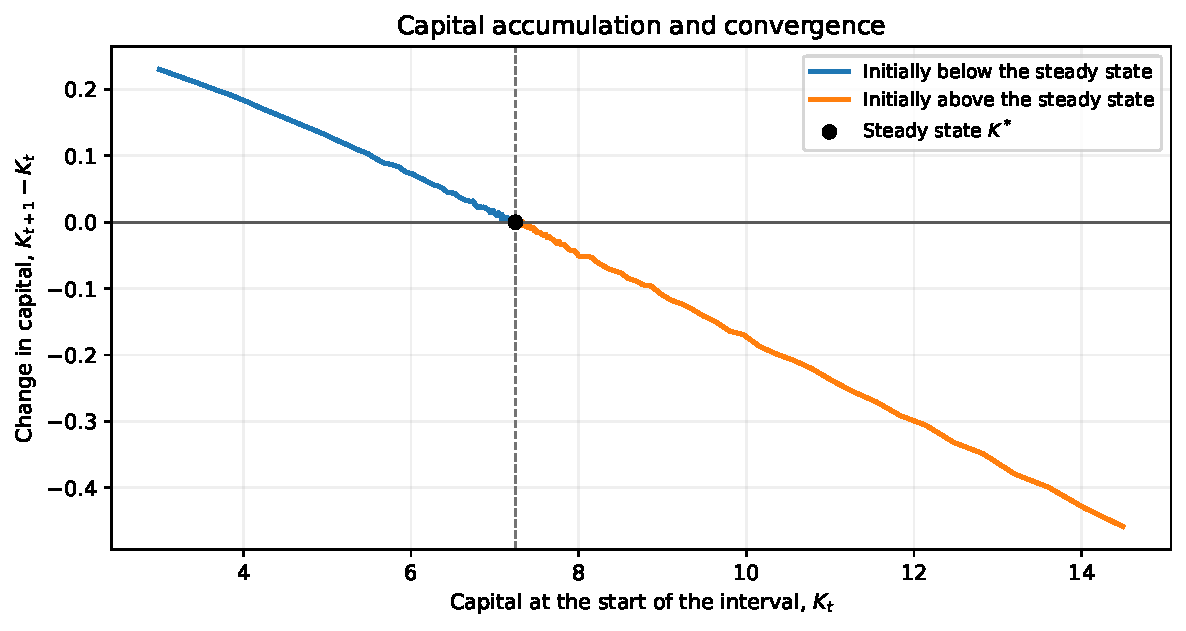
\includegraphics[width=0.78\linewidth]{images/phase_diagram.pdf} \par
{\footnotesize
$\alpha=0.30$, $\beta=1/(1+0.015)$, $\delta=0.06$, $\gamma=2$, $A=L=1$, $\Delta=1$.\par
Same calibration and solver as the notebook; $K_0=3$ and $K_0=2K^*$.
}%

%TCIMACRO{\TeXButton{Transition: Box Out}{\transboxout}}%
%BeginExpansion
\transboxout
%EndExpansion%
%TCIMACRO{\TeXButton{EndFrame}{\end{frame}}}%
%BeginExpansion
\end{frame}%
%EndExpansion
%

%TCIMACRO{\TeXButton{BeginFrame}{\begin{frame}}}%
%BeginExpansion
\begin{frame}%
%EndExpansion
%

%TCIMACRO{\QTR{frametitle}{Optimal growth problem: Diagram Interpretation}}%
%BeginExpansion
\frametitle{Optimal growth problem: Diagram Interpretation}%
%EndExpansion


\textbf{Interpretation:}

\begin{itemize}
\item Case $K_{0}\leq\bar{K}$

\begin{itemize}
\item Capital is too low relative to its steady-state.

\item This requires higher investment (a larger share of output devoted to
$I_{t}$) and thus lower consumption in the short run and capital accumulates
$\Delta K>0$

\item Over time, capital rises toward $\bar{K}$.
\end{itemize}

\item Case $K_{0}\geq\bar{K}$

\begin{itemize}
\item Opposite mechanism: overaccumulation of capital $\rightarrow$ more consumption.

\item Depreciation dominates $\Delta K<0$
\end{itemize}

\item Case $K_{0}=\bar{K}$

\begin{itemize}
\item $\Delta K$ capital stock stationary. Consumption and investment stable.
\end{itemize}
\end{itemize}

If you want the proof of convergence with saddle path see:
[\href{https://olivierloisel.com/macroeconomics/Chapter\%202.pdf}{Lecture II}]%

%TCIMACRO{\TeXButton{Transition: Box Out}{\transboxout}}%
%BeginExpansion
\transboxout
%EndExpansion%
%TCIMACRO{\TeXButton{EndFrame}{\end{frame}}}%
%BeginExpansion
\end{frame}%
%EndExpansion


\subsection{The bruteforce approach}%

%TCIMACRO{\TeXButton{BeginFrame}{\begin{frame}}}%
%BeginExpansion
\begin{frame}%
%EndExpansion
%

%TCIMACRO{\QTR{frametitle}{Control Problem: a sketch of the numerical solution
%I}}%
%BeginExpansion
\frametitle{Control Problem: a sketch of the numerical solution I}%
%EndExpansion


\begin{itemize}
\item Because the social welfare is forward looking, the system is both
forward and backward looking as follows:%
\[
s_{t}=\arg\min_{\{s_{t}\}_{i\geq0}}-\sum_{i=0}^{\infty}(1+\rho)^{-i}%
L_{t+i}\,u(c_{t+i})
\]


\item When a sequence $\{s_{t+i}\}_{i=0}^{\infty}$ is found, one can compute:
\begin{align*}
x_{t}  &  =g(x_{t-1}),\qquad\text{\ \ \ \ \ \ \ \ \ }g:\ \mathbb{R}^{N_{x}%
}\rightarrow\mathbb{R}^{N_{x}},\\[0.3em]
y_{t}  &  =f\big(y_{t-1},\,x_{t},\,z_{t}\big),\qquad f:\ \mathbb{R}^{N_{y}%
}\times\mathbb{R}^{N_{x}}\times\mathbb{R}^{2}\rightarrow\mathbb{R}^{N_{y}}.
\end{align*}


\item $x_{t}\in\mathbb{R}^{N_{x}}$: \textbf{exogenous variables}
($A_{t},\ L_{t}$).

\item $y_{t}\in\mathbb{R}^{N_{y}}$: \textbf{endogenous states/flows}
($c_{t},Y_{t},K_{t}$).

\item $z_{t}=[s_{t}]^{\prime}\in\mathbb{R}$: \textbf{decision variables} (saving).
\end{itemize}

%

%TCIMACRO{\TeXButton{Transition: Box Out}{\transboxout}}%
%BeginExpansion
\transboxout
%EndExpansion%
%TCIMACRO{\TeXButton{EndFrame}{\end{frame}}}%
%BeginExpansion
\end{frame}%
%EndExpansion
%

%TCIMACRO{\TeXButton{BeginFrame}{\begin{frame}}}%
%BeginExpansion
\begin{frame}%
%EndExpansion
%

%TCIMACRO{\QTR{frametitle}{Control Problem: a sketch of the numerical solution
%II}}%
%BeginExpansion
\frametitle{Control Problem: a sketch of the numerical solution II}%
%EndExpansion


\begin{itemize}
\item \textbf{Idea.} Approximate the \textbf{infinite-horizon} objective with
a \textbf{finite} one. Let $\beta\equiv(1+\rho)^{-1}$. Because $\lim
_{i\rightarrow\infty}\beta^{i}=0$, the tail contributes little.

\item \textbf{Pick the horizon $I^{\star}$ }so that the tail weight is below a
tolerance $\varepsilon$:
\[
\beta^{\,I^{\star}}\leq\varepsilon\quad
%\Longrightarrow\quad I^{\star}\;\geq\;\Big\lceil\frac{\ln\varepsilon}{\ln\beta_{\Delta}}\Big\rceil.
\]
\emph{Trade-off:} smaller $I^{\star}$ $\Rightarrow$ faster solve but larger
truncation error.

\item \textbf{Finite-horizon problem }that solves
\[
\max_{\{s_{t+i},\,\mu_{t+i}\}_{i=0}^{I^{\star}}}\;\sum_{i=0}^{I^{\star}}%
\beta^{\,i}\,L_{t+i}\,U\left(  \,c_{t+i}\right)  \;
\]%
\[
\text{s.t. (resource, capital) and bounds.}%
\]

\end{itemize}

%

%TCIMACRO{\TeXButton{Transition: Box Out}{\transboxout}}%
%BeginExpansion
\transboxout
%EndExpansion%
%TCIMACRO{\TeXButton{EndFrame}{\end{frame}}}%
%BeginExpansion
\end{frame}%
%EndExpansion
%

%TCIMACRO{\TeXButton{BeginFrame}{\begin{frame}}}%
%BeginExpansion
\begin{frame}%
%EndExpansion


\begin{center}
Thank you!

\vspace{5ex}

$gauthier.vermandel@polytechnique.edu$
\end{center}

%

%TCIMACRO{\TeXButton{Transition: Box Out}{\transboxout}}%
%BeginExpansion
\transboxout
%EndExpansion%
%TCIMACRO{\TeXButton{EndFrame}{\end{frame}}}%
%BeginExpansion
\end{frame}%
%EndExpansion
%

%TCIMACRO{\TeXButton{FRAME}{\bibliographystyle{apalike}
%\bibliography{lucas_romie}}}%
%BeginExpansion
\bibliographystyle{apalike}
\bibliography{lucas_romie}%
%EndExpansion

\end{document}
